
%% bare_conf.tex
%% V1.4b
%% 2015/08/26
%% by Michael Shell
%% See:
%% http://www.michaelshell.org/
%% for current contact information.
%%
%% This is a skeleton file demonstrating the use of IEEEtran.cls
%% (requires IEEEtran.cls version 1.8b or later) with an IEEE
%% conference paper.
%%
%% Support sites:
%% http://www.michaelshell.org/tex/ieeetran/
%% http://www.ctan.org/pkg/ieeetran
%% and
%% http://www.ieee.org/

%%*************************************************************************
%% Legal Notice:
%% This code is offered as-is without any warranty either expressed or
%% implied; without even the implied warranty of MERCHANTABILITY or
%% FITNESS FOR A PARTICULAR PURPOSE! 
%% User assumes all risk.
%% In no event shall the IEEE or any contributor to this code be liable for
%% any damages or losses, including, but not limited to, incidental,
%% consequential, or any other damages, resulting from the use or misuse
%% of any information contained here.
%%
%% All comments are the opinions of their respective authors and are not
%% necessarily endorsed by the IEEE.
%%
%% This work is distributed under the LaTeX Project Public License (LPPL)
%% ( http://www.latex-project.org/ ) version 1.3, and may be freely used,
%% distributed and modified. A copy of the LPPL, version 1.3, is included
%% in the base LaTeX documentation of all distributions of LaTeX released
%% 2003/12/01 or later.
%% Retain all contribution notices and credits.
%% ** Modified files should be clearly indicated as such, including  **
%% ** renaming them and changing author support contact information. **
%%*************************************************************************


% *** Authors should verify (and, if needed, correct) their LaTeX system  ***
% *** with the testflow diagnostic prior to trusting their LaTeX platform ***
% *** with production work. The IEEE's font choices and paper sizes can   ***
% *** trigger bugs that do not appear when using other class files.       ***                          ***
% The testflow support page is at:
% http://www.michaelshell.org/tex/testflow/



\documentclass[conference]{IEEEtran}
% Some Computer Society conferences also require the compsoc mode option,
% but others use the standard conference format.
%
% If IEEEtran.cls has not been installed into the LaTeX system files,
% manually specify the path to it like:
% \documentclass[conference]{../sty/IEEEtran}





% Some very useful LaTeX packages include:
% (uncomment the ones you want to load)


% *** MISC UTILITY PACKAGES ***
%
%\usepackage{ifpdf}
% Heiko Oberdiek's ifpdf.sty is very useful if you need conditional
% compilation based on whether the output is pdf or dvi.
% usage:
% \ifpdf
%   % pdf code
% \else
%   % dvi code
% \fi
% The latest version of ifpdf.sty can be obtained from:
% http://www.ctan.org/pkg/ifpdf
% Also, note that IEEEtran.cls V1.7 and later provides a builtin
% \ifCLASSINFOpdf conditional that works the same way.
% When switching from latex to pdflatex and vice-versa, the compiler may
% have to be run twice to clear warning/error messages.






% *** CITATION PACKAGES ***
%
%\usepackage{cite}
% cite.sty was written by Donald Arseneau
% V1.6 and later of IEEEtran pre-defines the format of the cite.sty package
% \cite{} output to follow that of the IEEE. Loading the cite package will
% result in citation numbers being automatically sorted and properly
% "compressed/ranged". e.g., [1], [9], [2], [7], [5], [6] without using
% cite.sty will become [1], [2], [5]--[7], [9] using cite.sty. cite.sty's
% \cite will automatically add leading space, if needed. Use cite.sty's
% noadjust option (cite.sty V3.8 and later) if you want to turn this off
% such as if a citation ever needs to be enclosed in parenthesis.
% cite.sty is already installed on most LaTeX systems. Be sure and use
% version 5.0 (2009-03-20) and later if using hyperref.sty.
% The latest version can be obtained at:
% http://www.ctan.org/pkg/cite
% The documentation is contained in the cite.sty file itself.






% *** GRAPHICS RELATED PACKAGES ***
%
\ifCLASSINFOpdf
  \usepackage[pdftex]{graphicx}
  % declare the path(s) where your graphic files are
  \graphicspath{{../pdf/}{../jpeg/}}
  % and their extensions so you won't have to specify these with
  % every instance of \includegraphics
  \DeclareGraphicsExtensions{.pdf,.jpeg,.png}
\else
  % or other class option (dvipsone, dvipdf, if not using dvips). graphicx
  % will default to the driver specified in the system graphics.cfg if no
  % driver is specified.
  \usepackage[dvips]{graphicx}
  % declare the path(s) where your graphic files are
  \graphicspath{{../eps/}}
  % and their extensions so you won't have to specify these with
  % every instance of \includegraphics
  \DeclareGraphicsExtensions{.eps}
\fi
% graphicx was written by David Carlisle and Sebastian Rahtz. It is
% required if you want graphics, photos, etc. graphicx.sty is already
% installed on most LaTeX systems. The latest version and documentation
% can be obtained at: 
% http://www.ctan.org/pkg/graphicx
% Another good source of documentation is "Using Imported Graphics in
% LaTeX2e" by Keith Reckdahl which can be found at:
% http://www.ctan.org/pkg/epslatex
%
% latex, and pdflatex in dvi mode, support graphics in encapsulated
% postscript (.eps) format. pdflatex in pdf mode supports graphics
% in .pdf, .jpeg, .png and .mps (metapost) formats. Users should ensure
% that all non-photo figures use a vector format (.eps, .pdf, .mps) and
% not a bitmapped formats (.jpeg, .png). The IEEE frowns on bitmapped formats
% which can result in "jaggedy"/blurry rendering of lines and letters as
% well as large increases in file sizes.
%
% You can find documentation about the pdfTeX application at:
% http://www.tug.org/applications/pdftex





% *** MATH PACKAGES ***
%
\usepackage{amsmath}
% A popular package from the American Mathematical Society that provides
% many useful and powerful commands for dealing with mathematics.
%
% Note that the amsmath package sets \interdisplaylinepenalty to 10000
% thus preventing page breaks from occurring within multiline equations. Use:
%\interdisplaylinepenalty=2500
% after loading amsmath to restore such page breaks as IEEEtran.cls normally
% does. amsmath.sty is already installed on most LaTeX systems. The latest
% version and documentation can be obtained at:
% http://www.ctan.org/pkg/amsmath





% *** SPECIALIZED LIST PACKAGES ***
%
%\usepackage{algorithmic}
% algorithmic.sty was written by Peter Williams and Rogerio Brito.
% This package provides an algorithmic environment fo describing algorithms.
% You can use the algorithmic environment in-text or within a figure
% environment to provide for a floating algorithm. Do NOT use the algorithm
% floating environment provided by algorithm.sty (by the same authors) or
% algorithm2e.sty (by Christophe Fiorio) as the IEEE does not use dedicated
% algorithm float types and packages that provide these will not provide
% correct IEEE style captions. The latest version and documentation of
% algorithmic.sty can be obtained at:
% http://www.ctan.org/pkg/algorithms
% Also of interest may be the (relatively newer and more customizable)
% algorithmicx.sty package by Szasz Janos:
% http://www.ctan.org/pkg/algorithmicx




% *** ALIGNMENT PACKAGES ***
%
%\usepackage{array}
% Frank Mittelbach's and David Carlisle's array.sty patches and improves
% the standard LaTeX2e array and tabular environments to provide better
% appearance and additional user controls. As the default LaTeX2e table
% generation code is lacking to the point of almost being broken with
% respect to the quality of the end results, all users are strongly
% advised to use an enhanced (at the very least that provided by array.sty)
% set of table tools. array.sty is already installed on most systems. The
% latest version and documentation can be obtained at:
% http://www.ctan.org/pkg/array


% IEEEtran contains the IEEEeqnarray family of commands that can be used to
% generate multiline equations as well as matrices, tables, etc., of high
% quality.




% *** SUBFIGURE PACKAGES ***
\ifCLASSOPTIONcompsoc
  \usepackage[caption=false,font=normalsize,labelfont=sf,textfont=sf]{subfig}
\else
  \usepackage[caption=false,font=footnotesize]{subfig}
\fi
% subfig.sty, written by Steven Douglas Cochran, is the modern replacement
% for subfigure.sty, the latter of which is no longer maintained and is
% incompatible with some LaTeX packages including fixltx2e. However,
% subfig.sty requires and automatically loads Axel Sommerfeldt's caption.sty
% which will override IEEEtran.cls' handling of captions and this will result
% in non-IEEE style figure/table captions. To prevent this problem, be sure
% and invoke subfig.sty's "caption=false" package option (available since
% subfig.sty version 1.3, 2005/06/28) as this is will preserve IEEEtran.cls
% handling of captions.
% Note that the Computer Society format requires a larger sans serif font
% than the serif footnote size font used in traditional IEEE formatting
% and thus the need to invoke different subfig.sty package options depending
% on whether compsoc mode has been enabled.
%
% The latest version and documentation of subfig.sty can be obtained at:
% http://www.ctan.org/pkg/subfig




% *** FLOAT PACKAGES ***
%
%\usepackage{fixltx2e}
% fixltx2e, the successor to the earlier fix2col.sty, was written by
% Frank Mittelbach and David Carlisle. This package corrects a few problems
% in the LaTeX2e kernel, the most notable of which is that in current
% LaTeX2e releases, the ordering of single and double column floats is not
% guaranteed to be preserved. Thus, an unpatched LaTeX2e can allow a
% single column figure to be placed prior to an earlier double column
% figure.
% Be aware that LaTeX2e kernels dated 2015 and later have fixltx2e.sty's
% corrections already built into the system in which case a warning will
% be issued if an attempt is made to load fixltx2e.sty as it is no longer
% needed.
% The latest version and documentation can be found at:
% http://www.ctan.org/pkg/fixltx2e


%\usepackage{stfloats}
% stfloats.sty was written by Sigitas Tolusis. This package gives LaTeX2e
% the ability to do double column floats at the bottom of the page as well
% as the top. (e.g., "\begin{figure*}[!b]" is not normally possible in
% LaTeX2e). It also provides a command:
%\fnbelowfloat
% to enable the placement of footnotes below bottom floats (the standard
% LaTeX2e kernel puts them above bottom floats). This is an invasive package
% which rewrites many portions of the LaTeX2e float routines. It may not work
% with other packages that modify the LaTeX2e float routines. The latest
% version and documentation can be obtained at:
% http://www.ctan.org/pkg/stfloats
% Do not use the stfloats baselinefloat ability as the IEEE does not allow
% \baselineskip to stretch. Authors submitting work to the IEEE should note
% that the IEEE rarely uses double column equations and that authors should try
% to avoid such use. Do not be tempted to use the cuted.sty or midfloat.sty
% packages (also by Sigitas Tolusis) as the IEEE does not format its papers in
% such ways.
% Do not attempt to use stfloats with fixltx2e as they are incompatible.
% Instead, use Morten Hogholm'a dblfloatfix which combines the features
% of both fixltx2e and stfloats:
%
% \usepackage{dblfloatfix}
% The latest version can be found at:
% http://www.ctan.org/pkg/dblfloatfix




% *** PDF, URL AND HYPERLINK PACKAGES ***
%
%\usepackage{url}
% url.sty was written by Donald Arseneau. It provides better support for
% handling and breaking URLs. url.sty is already installed on most LaTeX
% systems. The latest version and documentation can be obtained at:
% http://www.ctan.org/pkg/url
% Basically, \url{my_url_here}.




% *** Do not adjust lengths that control margins, column widths, etc. ***
% *** Do not use packages that alter fonts (such as pslatex).         ***
% There should be no need to do such things with IEEEtran.cls V1.6 and later.
% (Unless specifically asked to do so by the journal or conference you plan
% to submit to, of course. )


% correct bad hyphenation here
\hyphenation{}


\begin{document}
%
% paper title
% Titles are generally capitalized except for words such as a, an, and, as,
% at, but, by, for, in, nor, of, on, or, the, to and up, which are usually
% not capitalized unless they are the first or last word of the title.
% Linebreaks \\ can be used within to get better formatting as desired.
% Do not put math or special symbols in the title.
\title{A graph-based data model for interactive 
evolutionary computation}


% author names and affiliations
% use a multiple column layout for up to three different
% affiliations
\author{\IEEEauthorblockN{Michael Shell}
\IEEEauthorblockA{School of Electrical and\\Computer Engineering\\
Georgia Institute of Technology\\
Atlanta, Georgia 30332--0250\\
Email: http://www.michaelshell.org/contact.html}
\and
\IEEEauthorblockN{Homer Simpson}
\IEEEauthorblockA{Twentieth Century Fox\\
Springfield, USA\\
Email: homer@thesimpsons.com}
\and
\IEEEauthorblockN{James Kirk\\ and Montgomery Scott}
\IEEEauthorblockA{Starfleet Academy\\
San Francisco, California 96678--2391\\
Telephone: (800) 555--1212\\
Fax: (888) 555--1212}}




% make the title area
\maketitle

% As a general rule, do not put math, special symbols or citations
% in the abstract
\begin{abstract}
This paper presents an alternative data model for the development of
Interactive Evolutionary Computation (IEC) algorithms. A graph %specify
                                %the elements of the graph - JJ
stored for efficiency in a graph database, is
proposed to model the overall system which consists of: a social network of
volunteers participating in the interactive evolutionary experiment, a
population of individuals in the evolutionary algorithm, 
the system\'s functionality and their interactions. This graph model can then be used
to tackle some of the issues associated with IEC such as, 
user fatigue, lack of volunteer participation, fitness estimation % what is this issue?
%Maybe the abstract should start with the issues we want to tackle as
%motivation. Motivation always goes first - JJ
and novelty. % These two last issues are not too clear, maybe they
             % could be explained in that motivation. 
The proposed graph database could be used to model IEC systems that 
follow a user-centered approach. % Graph is the model, graph database
                                % the implementation. Two different
                                % things. 
A case study is presented providing both 
conceptual and implementation details using the EvoSpace-Interactive
platform.
% It must prove that the issues have been addressed - JJ
\end{abstract}

% no keywords




% For peer review papers, you can put extra information on the cover
% page as needed:
% \ifCLASSOPTIONpeerreview
% \begin{center} \bfseries EDICS Category: 3-BBND \end{center}
% \fi
%
% For peerreview papers, this IEEEtran command inserts a page break and
% creates the second title. It will be ignored for other modes.
\IEEEpeerreviewmaketitle



\section{Introduction}
% Maybe an introduction on why and where to use these types of
% algorithms? - jj
% Done -Mario
Interactive Evolutionary Algorithms (IEAs) are standard EAs whose
fitness evaluations are performed by persons within an interactive 
system.  Thus, the main loop of the EA needs the intervention of a
human for the quality assessment of each proposed solution.
IEAs have demonstrated their ability for effectively
producing art and design \cite{Bentley:1999:intro,Sims:1991,todd:1992},
as well as other products in many other domains \cite{ie1}. 
Several IECs have been developed as web based systems \cite{picbreeder},
who depend on volunteers who visit the system to interactively help
with the search, using both anonymous and registered users.
These systems have several inherent drawbacks arising from the very nature of 
the algorithms, namely, the human fatigue caused by the interaction, and
the boredom arising when users evaluate a large number of individuals 
many of which are not interesting or are very similar to each other.
IEAs also share some of the issues commonly found in volunteer based systems
\cite{sarmenta2001volunteer,web:BOINC} such as the volunteer\'s lack of accountability,
and the need to build trust between participants and application providers. 
For the provider there is also the difficulty of establishing 
the amount of time and resources
a volunteer is willing to spend on the system, and how they decide if they
participate or not \cite{JJ:2016}. In order to increase participation and 
engagement, and to tackle the issues mentioned above,  
IEAs must follow a user centered design, giving extensive attention 
to volunteer users, not only because their
explicit evaluation is essential, but also because the context of the 
interaction affects the system as a whole. Users interact not only with the graphical
interface, and each individual\'s phenotype, there is also the interaction
with other users, their previous evaluations and their own stream of activities
and past experiences. Thus users in this proposal are defined as dynamic entities 
interacting with an evolutionary computation having the fundamental purpose 
of evaluating individuals according to their preferences,
both explicitly or implicitly. In this work we propose giving the same
importance to users and their interactions as the population of 
individuals have in a traditional EA, even to the extend as using this
knowledge as an integral part of the algorithm it self. We argue also
that a graph model is a viable representation for this purpose,  
presenting a natural way of maping the relationships found in the system. 
Most IEAs can have the following many-to-many relations:

\begin{itemize}
  \item { \tt Individual-Individual} The relationship between individuals 
  is naturally expressed as a tree, or a graph when both ancestors 
  and descendants is considered. Other semantic relations can also be considered
  for instance: similarity or composition.

  \item {\tt User-Individual}
  Many kinds of relationships between users and individuals,
  can be expressed using common actions found in social networks;
  for instance share, like, rate or add to collection [cite Activity Streams 2.0
  syntax (https://www.w3.org/TR/activitystreams-vocabulary)]. In IEAs these
  relationships are used to assigned a single or a collection of
  fitness values to individuals [cite ES-I].   

  \item {\tt User-User}
  Relationship between users can also be modeled 
  as a social network, with well stablished algorithms and metrics (cite).
  Identifyng leaders of opinion and the similarity between user\'s 
  preferences is of special importance for IEAs, as they could be used
  to recommend to users only those individuals they will probably like more. 

\end{itemize}

These relations are naturaly maped to graphs, while other actions and 
properties can also be modeled as a semantic network using
basic subject–-predicate-–object expressions [cite Semantic triples].
Another reason for using a graph model is the tools available for
implementing and query the model, and the increased performance of
native graph database systems [cite Christian].


% Moving to related work - Mario
%\cite{Performance for the masses and Christian's previous work}, 



 % Can it be quantified? Maybe a reference to NodIO? - JJ
%Some authors have already tried to address this basic problem
%\cite{Frade:2010:EvoGAMES}. %Non sequitur. Is it something we are
                            %going to do here? - jj
%% Moving this to Related Work Section -Mario

% Maybe this claim should go to the beginning. THIS is why we want to
% use them - JJ
% Done - Mario
 
A case study is presented as a proof of concept, providing both 
conceptual and implementation details of a graph data model for
the implementation of an IEA in the EvoSpace-Interactive platform. 
The graph database is then used to measure the degree of relationship
between users and their participation.  

The remainder of this paper is organized  as follows.
Section \ref{sec:interactive} presents related work on the topic 
of Interactive Evolution data models.
Then, Section \ref{sec:evospace-i} presents the computational platform on which 
the main proposal of this work is developed. The proposed graph model is 
presented in Section \ref{sec:graph}.
The experimental work and results are presented in Section \ref{sec:experiments}.
Finally, a concluding remarks are provided in Section \ref{sec:conclusions}.


\section{Related Work}
\label{sec:interactive}

\section{EvoSpace-Interactive}
\label{sec:evospace-i} 
As a case study, a IEA was implented using the 
EvoSpace-Interactive (ES-I) platform \cite{garcia2013evospace}. %citation
A brief description of the aplication is presented next, focusing
on the data elements that where ported to the graph model.

\subsection{Fitness Assignment}
\label{sec:col}
The ES-I platform employs a collaborative technique,
where several registered users assign a quality assessment to a single
individual and then an aggregated fitness value is calculated. The fitness
assigned to each individual depends on the taste of each particular user, 
resulting in a many-to-many relationship between users and individuals. 
Many systems query this user-individual relation to extract relevant
knowledge about the process and the population, for instance showing the
most popular individual, or the the user with more participation \cite{picbreeder}.
In order to do this, data about individuals %what? Maybe data
                                %about individuals? - JJ
must be permanently stored, even
if they are no longer in the active population. 

\subsection{Collaboration}
\label{sec:col}
After entering the web application by using their Facebook account,
users can collaborate with their Facebook friends, 
sharing those individuals they like, or by taking individuals
from their friend\'s collections by using the web interface depicted 
in Figure \ref{fig:web}

\begin{figure*}
\captionsetup{justification=centering,margin=2cm}
\centering
\setlength\fboxsep{0pt}
\setlength\fboxrule{0.7pt}
\fbox{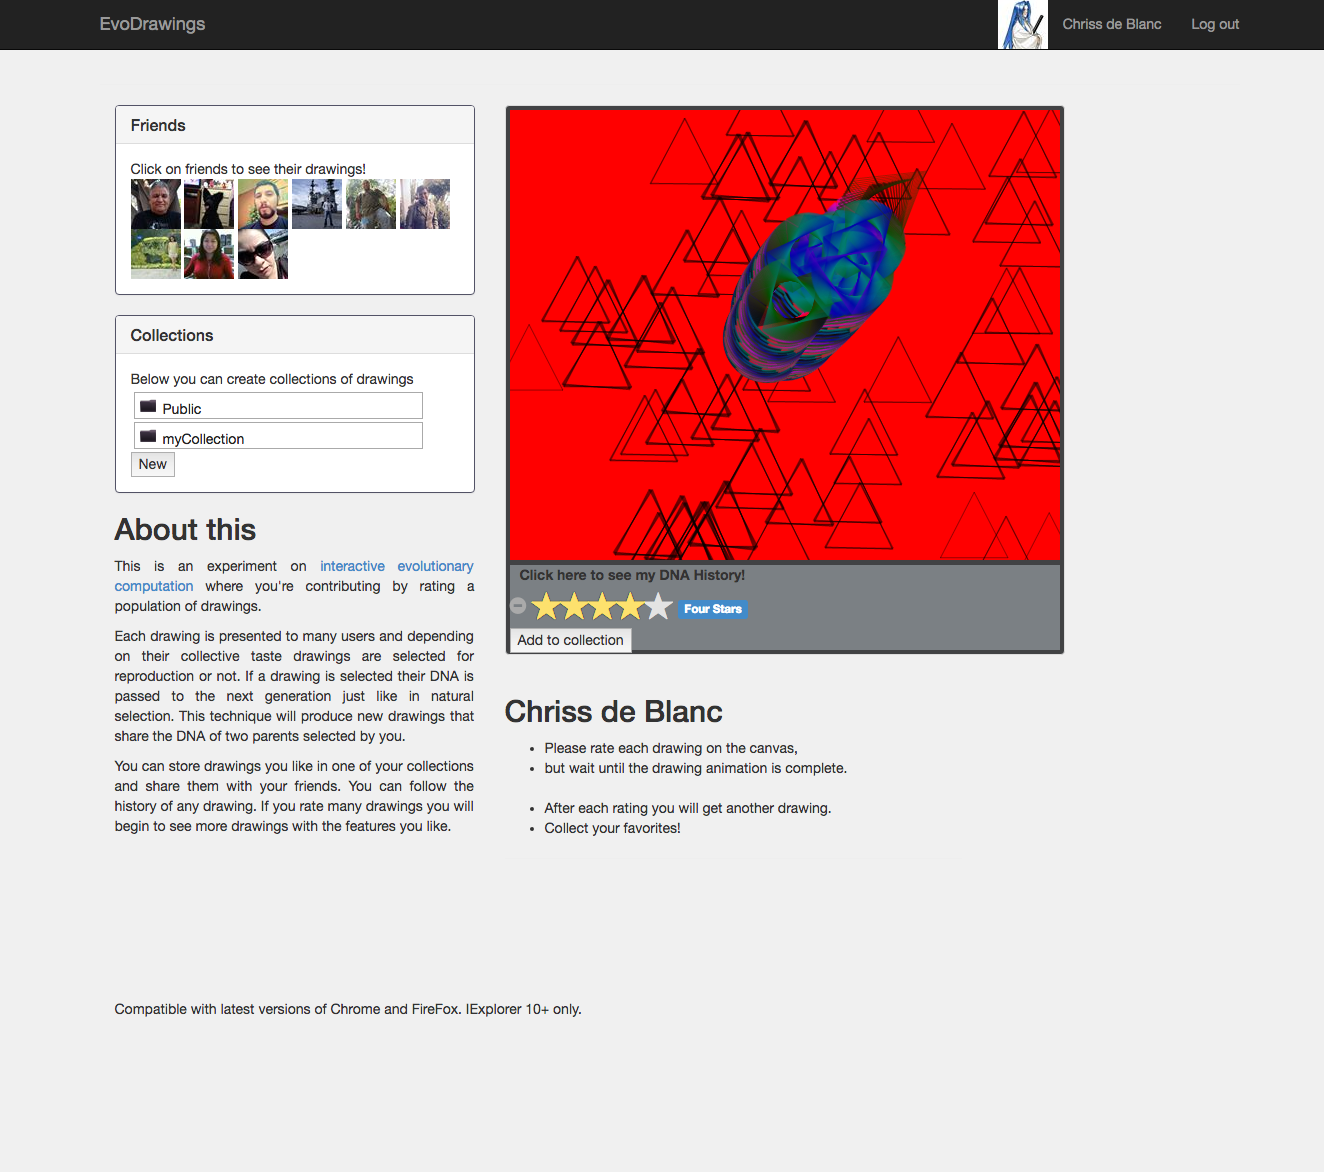
\includegraphics[width=12cm,height=10cm,keepaspectratio]{img/UI_ed01.png}}
\caption{User interface ED01.}
\label{fig:web}       
\end{figure*}

At the top left corner list of Facebook friends is presented, 
to encourage users to interact with the system. In the central 
\emph{ Wall } area, an individual sampled from the population 
is shown to the user.
Here, the user can interact with the system in two ways.
He can assign a quality assessment to the individual using
a five star rating measure.
Additionally, a user can choose to add an image to one of their \emph{Collections}.
A collection is a special directory to store individuals a user prefers and wishes
to save. After the user finishes interacting the individual
on the Wall, he can choose to retrieve a new one from population.
At the left side, is the \emph{Collections} section.
The user can create several collections, to group and organize his favorite 
artifacts. Moreover, a user can browse the content of each collection and from
there share images through the social network.
When a user browses over an individual a detail pane shows how many users have
liked the individual. The pane also includes a link to the individual's 
details, the parents, genetic operators that created it, and genealogy information.
 
\section{IEC Graph based model}
\label{sec:graph}
The fundamental goal of this research is to develop a user-centered framework
for interactive evolutionary computation (IEC) in order to increase users’
participation and also to minimize the amount of evaluations needed for the
evolutionary process in given Web-based IEC application.

In this chapter an explanation of the proposed framework is described. The
different techniques used, such as user modeling, fuzzy logic, and human-
interaction.

This framework is presented in figure \ref{fig:uc_framework}. Each of the
entities of this framework will be explained in detail in following sections.

The current model is tailored to the EvoSpace-I functionality and capabilities
but it can be modified to handle other platforms, just by adding new clases 
of nodes.


\begin{figure*}
  \captionsetup{justification=centering,margin=2cm}
  \centering
  \setlength\fboxsep{0pt}
  \setlength\fboxrule{0.7pt}
  \fbox{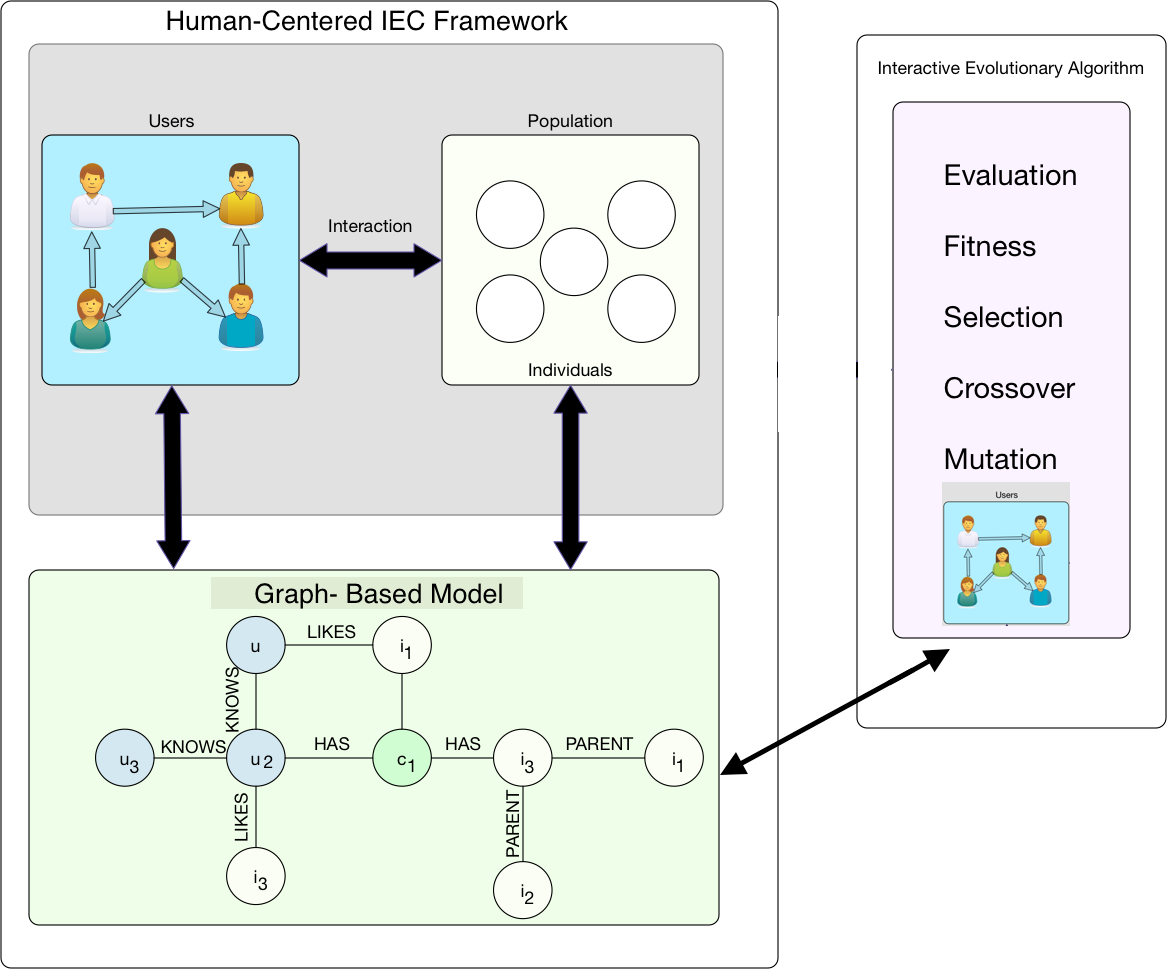
\includegraphics[width=10cm,height=10cm,keepaspectratio]{img/framework.png}}
  \caption{User-Centerd Framework.}
  \label{fig:uc_framework}       
\end{figure*}

%A hint on how
% done -Mario

\subsection{Users} 

In this sense the action of posting is when
users want to put something on their wall who want others to know through
their social networks. Likewise the storing action occurs when users want to
retain permanently information that are of their interest. Finally the
browsing action occurs when users are exploring content for their needs. All
these actions go beyond only evaluating individuals.

\begin{figure*}
  \captionsetup{justification=centering,margin=2cm}
  \centering
  \setlength\fboxsep{0pt}
  \setlength\fboxrule{0.7pt}
  \fbox{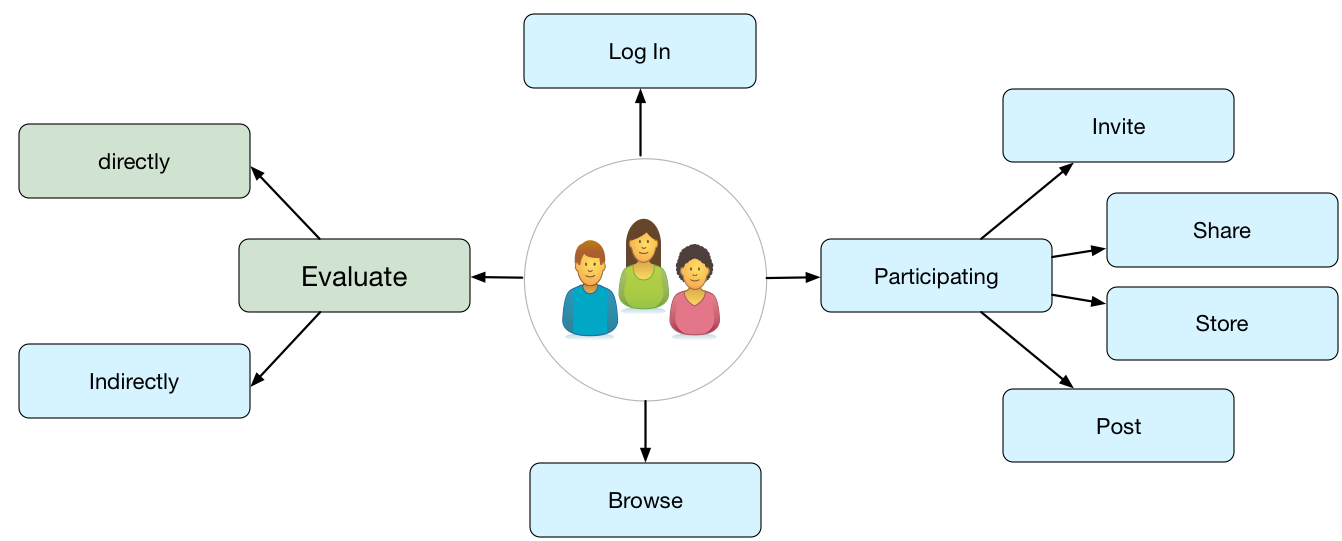
\includegraphics[width=10cm,height=10cm,keepaspectratio]{img/users.png}}
  \caption{Users actions on interactive evolutionary systems.}
  \label{fig:users}       
\end{figure*}

In order to start the task of evaluating individuals is necessary that users
access the system through a login mechanism. This mechanism consists of
providing a username and a password in order to grant access to the system. All
users accessing in this way they are considered active users within an IEC
system.

For the evaluating action is proposed  that users evaluate individuals
indirectly, this means users can evaluate accepting indirect recommendations of
friends that are currently active in the system. These recommendations can be
store individuals in the system of users who know each other.

Also the  browsing action is proposed within IEC systems,  this means that users
can explore information that other active users in the system are generating.

Finally activity participation is proposed. This can be divided into four
different actions as fallows:

\begin{itemize} 
\item The Inviting action occurs when a user invites another to the system through social networks or from person to person.  
\item The sharing action occurs when users share their individual creations with others active user in the system.
\item The posting action occurs when published what they are doing within the system.
\item The storing action occurs when users keep individuals in a collection, the collections concept will be discussed later in this chapter.
\end{itemize}

All the mention above is shown in figure \ref{fig:users}

\subsection{Individual}  

Individuals are entities that form the population for the evolutionary
algorithm. In particular for  this work individuals are animated digital
paintings, every individual in the population is defined by a chromosome [].
This chromosome defines the behavior of the individual, so that it consists of a
vector of real numbers of fifteen genes, where each gen define a particular
behavior in painting. This individuals combined each other to generated new
individual in the population following the genetic operators such as selection,
crossover and mutation[]. 

\subsection{User Model} Now that both users an individuals have been defined we can
model the users behavior have with respect to individuals in a graph-based user
model.

The reason for using a graph to model the user-individual is because it could
can express in a simple way the behavior of this two entities having the
necessary information  to represent the knowledge,  for example a vertex user
and individual vertex connected through a edge that  represents the
relationship. this relationship can be the semantic  between these two entities
as figure \ref{fig:User-Individual} show. Each of these vertices contain properties as well as the
edges, these properties will be explained as fallows.

\begin{figure*}
\captionsetup{justification=centering,margin=2cm}
\centering
\setlength\fboxsep{0pt}
\setlength\fboxrule{0.7pt}
\fbox{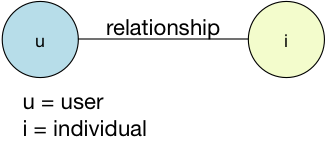
\includegraphics[width=5cm,height=5cm,keepaspectratio]{img/user_individual.png}}
\caption{User-Individual.}
\label{fig:User-Individual}       
\end{figure*}

In this proposed graph-based user-individual model the vertices are represented
by set of nodes of USERS, INDIVIDUALS and COLLECTIONS. The edges are define by a
set of relationships as LIKES, KNOWS, PARENT, HAS that represents the
relationships between the vertices as seen in figure \ref{fig:User-Individual}.

Already explained that represent USERS and INDIVIDUALS, now an explanation is
given of what concerns for the concept of COLLECTIONS.

In this proposal a collection is defined as a  container where users can store
selected individuals laid within the collection. A collection is created when
the user wants to store permanently individuals within the IEC system.

Now for the edges in this proposal are explained as follows:

\begin{itemize} 
\item The  LIKES edge represents a preference relationship that a user has with respect to an individual.  
\item Now the  PARENT edge represents an ancestor of the individual, in other words where the individual comes from.
\item Likewise the  HAS edge represents that users have a collection where can contain individuals.
\item Finally the KNOWS edge represents a relationship of friendship between users.
\end{itemize}

In figure \ref{fig:Nodes_Edges} illustrated the above mentioned, about nodes and edges.

\begin{figure*}
\captionsetup{justification=centering,margin=2cm}
\centering
\setlength\fboxsep{0pt}
\setlength\fboxrule{0.7pt}
\fbox{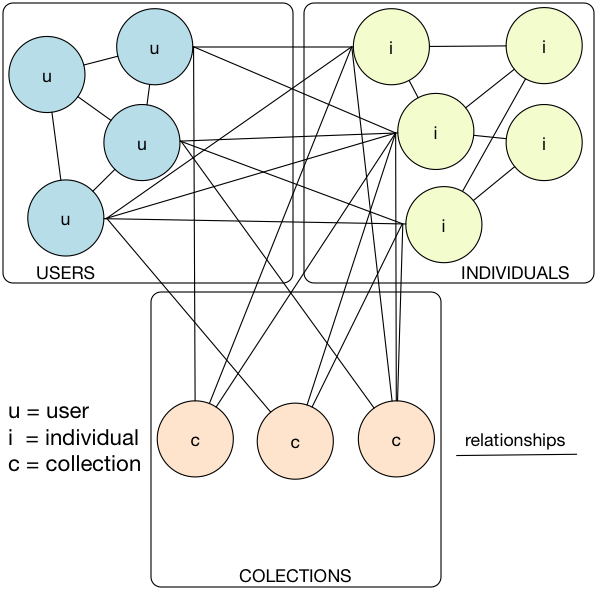
\includegraphics[width=10cm,height=10cm,keepaspectratio]{img/user_individual_collections.png}}
\caption{Nodes And Edges Representation.}
\label{fig:Nodes_Edges}       
\end{figure*}


In each vertex is necessary to store knowledge about the users, individuals and
also for the collections, this is what is known as property.

It is worth to mention that all vertices have a property called “element\_type”
among others. This property is used to identify which type of vertex is, for
example if vertex corresponds to a user then this property label the vertex as a
“person”. Likewise if the vertex corresponds to an individual this property
label it as an “individual” and is the same for any vertex we want to add to the
model. This property also has the purpose of being able to do operations on the
graph according to the vertex type.

The properties for the vertex “u” are the following:

\begin{itemize} 
\item id.  
\item created.
\item name.
\item element\_type.
\end{itemize}

The “id” property defines that the vertex u has a unique identifier in the set
of vertices, which means that there will not be duplicate vertices. The property
“created” defines the creation date of the vertex $u$. The property “name”
defines the name of the vertex u. The property “element\_type” defines the
element type that will be the vertex $u$.

In figure \ref{fig:User_node} the properties of vertex $u$  are shown.

\begin{figure*}
\captionsetup{justification=centering,margin=2cm}
\centering
\setlength\fboxsep{0pt}
\setlength\fboxrule{0.7pt}
\fbox{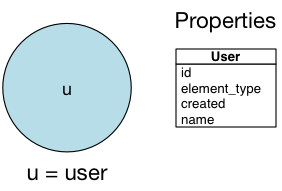
\includegraphics[width=5cm,height=5cm,keepaspectratio]{img/user_node.png}}
\caption{User Properties.}
\label{fig:User_node}       
\end{figure*}

The properties for the vertex $i$ are the following:
\begin{itemize} 
\item id. 
\item created. 
\item element\_type.
\item chromosome.
\item views.
\end{itemize}

The “id” property defines that the vertex $i$ has a unique identifier in the set
of vertices, which means that there will not be duplicate vertices. The
“chromosome” property defines the chromosome of the individual representing the
vertex $i$. which as defined above in this section. The  property “views” defines
the amount that users have seen this vertex $i$ The property “element\_type”
defines the element type that will be the vertex $i$. The property “created”
defines the creation date of the vertex $i$. % Is there a point in
                                % describing these properties? - JJ


In figure \ref{fig:Individual_node} the vertex $i$ properties are shown.

\begin{figure*}
\captionsetup{justification=centering,margin=2cm}
\centering
\setlength\fboxsep{0pt}
\setlength\fboxrule{0.7pt}
\fbox{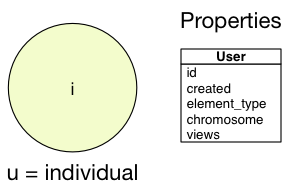
\includegraphics[width=5cm,height=5cm,keepaspectratio]{img/individual_node.png}}
\caption{Individual Properties.}
\label{fig:Individual_node}       
\end{figure*}

The properties for the vertex “c” are the following:

\begin{itemize} 
\item id. 
\item element\_type.
\item created. 
\item name.
\end{itemize}

The “id” property defines that the vertex $c$ has a unique identifier in the set
of vertices, which means that there will not be duplicate vertices. The property
“element\_type” defines the element type that will be the vertex $c$. The
property “name” defines the name of the vertex $c$. The property “created”
defines the creation date of the vertex $c$.

In figure \ref{fig:Collection_node} the vertex $c$ properties are shown.

\begin{figure*}
\captionsetup{justification=centering,margin=2cm}
\centering
\setlength\fboxsep{0pt}
\setlength\fboxrule{0.7pt}
\fbox{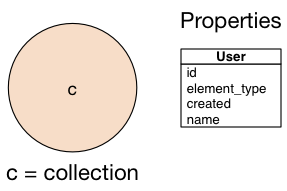
\includegraphics[width=5cm,height=5cm,keepaspectratio]{img/collection_node.png}}
\caption{Collection Properties.}
\label{fig:Collection_node}       
\end{figure*}

In the same way that the vertices have properties also the edges, these
properties are defined as follows.

The “LIKES” edge has the following properties:

\begin{itemize} 
\item id. 
\item created. 
\item rate.
\end{itemize}

The “id” property defines that the “LIKES” edge  has a unique identifier in the
set of edges, which means that there will not be duplicate edges. The property
“created” defines the date of creation of the this edge. The property “rate”
defines the rate that the users give to the individual store in this edge.

In figure \ref{fig:Likes_edge} the edge “LIKES” properties and the relationships with the vertices $u$ and $i$ are shown.


\begin{figure*}
\captionsetup{justification=centering,margin=2cm}
\centering
\setlength\fboxsep{0pt}
\setlength\fboxrule{0.7pt}
\fbox{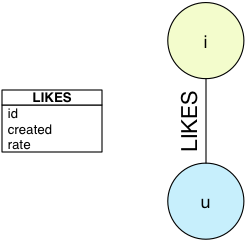
\includegraphics[width=5cm,height=5cm,keepaspectratio]{img/edge_properties_likes.png}}
\caption{LIKES edge Properties.}
\label{fig:Likes_edge}       
\end{figure*}

The “KNOWS” edge has the following properties.
\begin{itemize} 
\item id. 
\item created. 
\end{itemize}

The “id” property defines that the edge “KNOWS” has a unique identifier in the
set of edges, which means that there will not be duplicate edges. The property
“created” defines the date of creation of the edge.

In figure \ref{fig:Knows_edge} the edge “KNOWS” properties and the relationships between vertex “u”
are shown.

\begin{figure*}
\captionsetup{justification=centering,margin=2cm}
\centering
\setlength\fboxsep{0pt}
\setlength\fboxrule{0.7pt}
\fbox{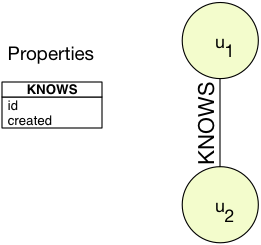
\includegraphics[width=5cm,height=5cm,keepaspectratio]{img/edge_properties_knows.png}}
\caption{KNOWS edge Properties.}
\label{fig:Knows_edge}       
\end{figure*}

The “PARENT” edge has the following properties, and represent the parents of a new individual.
\begin{itemize} 
\item id. 
\item created. 
\end{itemize}

The “id” property defines that the edge “PARENT” has a unique identifier in the set of edges, which means that there will not be duplicate edges.
The property “created” defines the date of creation of the edge.

In figure \ref{fig:Parent_edge} the edge “PARENT” properties and the relationship between vertex $i$ are shown.

\begin{figure*}
\captionsetup{justification=centering,margin=2cm}
\centering
\setlength\fboxsep{0pt}
\setlength\fboxrule{0.7pt}
\fbox{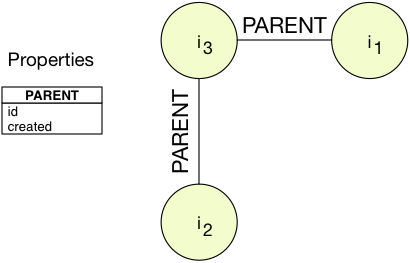
\includegraphics[width=5cm,height=5cm,keepaspectratio]{img/edge_properties_parent.png}}
\caption{PARENT edge Properties.}
\label{fig:Parent_edge}       
\end{figure*}

The edge “HAS” has the following properties, and represent the parents of a new individual.
\begin{itemize} 
\item id. 
\item created. 
\end{itemize}

The “id” property defines that the edge “HAS” has a unique identifier in the set of edges, which means that there will not be duplicate edges.
The property “created” defines the date of creation of the edge.

In figure \ref{fig:Has_edge} the edge “HAS” properties and the relationship between vertices $u$, $i$ and $c$ are shown.

\begin{figure*}
\captionsetup{justification=centering,margin=2cm}
\centering
\setlength\fboxsep{0pt}
\setlength\fboxrule{0.7pt}
\fbox{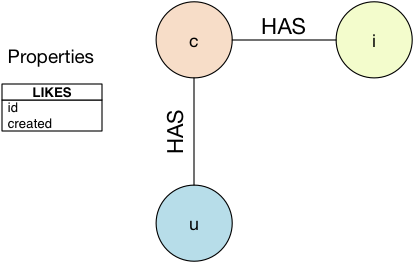
\includegraphics[width=5cm,height=5cm,keepaspectratio]{img/edge_properties_has.png}}
\caption{HAS edge Properties.}
\label{fig:Has_edge}       
\end{figure*}

\begin{equation*}\label{eq:graphRelDef} 
\displaystyle 
\begin{split} 
V &= \{[u_1,u_2,u_3,...,u_n],[i_1,i_2,i_3,...,i_n],[c_1,c_2,c_3,...,c_n]\},\\ 
E&= \{[l_1,l_2,l_3,..,l_n],[p_1,p_2,p_3,...,p_n],[h_1,h_2,h_3,...,h_n],[k_1,k_2,k_3,...,k_n]\}\\ 
\end{split} 
\end{equation*} 

Once  the vertices and edges have been defined a graph-based user-individual model is
proposed where  user vertices are related to the individual vertices, likewise
the vertices individuals are related to themselves when evolution exist between
them. % Grammar has to be improved - JJ
In that sense the vertices users and individuals are related to the
vertices collections as a vertex user can be related to a vertex collections and
a vertex collections collections is related to $n$ individuals vertex. In Figure
\ref{fig:user_moder} shows an example of the graph-based user-individual model.

\begin{figure*}
\captionsetup{justification=centering,margin=2cm}
\centering
\setlength\fboxsep{0pt}
\setlength\fboxrule{0.7pt}
\fbox{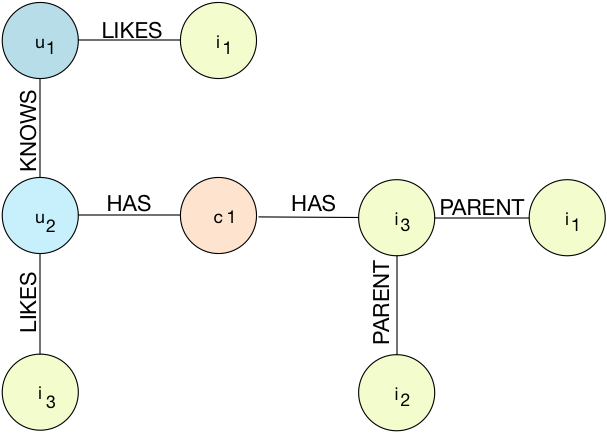
\includegraphics[width=8cm,height=8cm,keepaspectratio]{img/model_representation.png}}
\caption{Graph-based user-individual model.}
\label{fig:user_moder}       
\end{figure*}

\subsection{Experiments}
\label{sec:experiments}

\subsection{Conclusions}
\label{sec:conclusions}



% An example of a floating figure using the graphicx package.
% Note that \label must occur AFTER (or within) \caption.
% For figures, \caption should occur after the \includegraphics.
% Note that IEEEtran v1.7 and later has special internal code that
% is designed to preserve the operation of \label within \caption
% even when the captionsoff option is in effect. However, because
% of issues like this, it may be the safest practice to put all your
% \label just after \caption rather than within \caption{}.
%
% Reminder: the "draftcls" or "draftclsnofoot", not "draft", class
% option should be used if it is desired that the figures are to be
% displayed while in draft mode.
%
%\begin{figure}[!t]
%\centering
%\includegraphics[width=2.5in]{myfigure}
% where an .eps filename suffix will be assumed under latex, 
% and a .pdf suffix will be assumed for pdflatex; or what has been declared
% via \DeclareGraphicsExtensions.
%\caption{Simulation results for the network.}
%\label{fig_sim}
%\end{figure}

% Note that the IEEE typically puts floats only at the top, even when this
% results in a large percentage of a column being occupied by floats.


% An example of a double column floating figure using two subfigures.
% (The subfig.sty package must be loaded for this to work.)
% The subfigure \label commands are set within each subfloat command,
% and the \label for the overall figure must come after \caption.
% \hfil is used as a separator to get equal spacing.
% Watch out that the combined width of all the subfigures on a 
% line do not exceed the text width or a line break will occur.
%
%\begin{figure*}[!t]
%\centering
%\subfloat[Case I]{\includegraphics[width=2.5in]{box}%
%\label{fig_first_case}}
%\hfil
%\subfloat[Case II]{\includegraphics[width=2.5in]{box}%
%\label{fig_second_case}}
%\caption{Simulation results for the network.}
%\label{fig_sim}
%\end{figure*}
%
% Note that often IEEE papers with subfigures do not employ subfigure
% captions (using the optional argument to \subfloat[]), but instead will
% reference/describe all of them (a), (b), etc., within the main caption.
% Be aware that for subfig.sty to generate the (a), (b), etc., subfigure
% labels, the optional argument to \subfloat must be present. If a
% subcaption is not desired, just leave its contents blank,
% e.g., \subfloat[].


% An example of a floating table. Note that, for IEEE style tables, the
% \caption command should come BEFORE the table and, given that table
% captions serve much like titles, are usually capitalized except for words
% such as a, an, and, as, at, but, by, for, in, nor, of, on, or, the, to
% and up, which are usually not capitalized unless they are the first or
% last word of the caption. Table text will default to \footnotesize as
% the IEEE normally uses this smaller font for tables.
% The \label must come after \caption as always.
%
%\begin{table}[!t]
%% increase table row spacing, adjust to taste
%\renewcommand{\arraystretch}{1.3}
% if using array.sty, it might be a good idea to tweak the value of
% \extrarowheight as needed to properly center the text within the cells
%\caption{An Example of a Table}
%\label{table_example}
%\centering
%% Some packages, such as MDW tools, offer better commands for making tables
%% than the plain LaTeX2e tabular which is used here.
%\begin{tabular}{|c||c|}
%\hline
%One & Two\\
%\hline
%Three & Four\\
%\hline
%\end{tabular}
%\end{table}


% Note that the IEEE does not put floats in the very first column
% - or typically anywhere on the first page for that matter. Also,
% in-text middle ("here") positioning is typically not used, but it
% is allowed and encouraged for Computer Society conferences (but
% not Computer Society journals). Most IEEE journals/conferences use
% top floats exclusively. 
% Note that, LaTeX2e, unlike IEEE journals/conferences, places
% footnotes above bottom floats. This can be corrected via the
% \fnbelowfloat command of the stfloats package.




\section{Conclusion}
The conclusion goes here.




% conference papers do not normally have an appendix


% use section* for acknowledgment
\section*{Acknowledgment}


The authors would like to thank...





% trigger a \newpage just before the given reference
% number - used to balance the columns on the last page
% adjust value as needed - may need to be readjusted if
% the document is modified later
%\IEEEtriggeratref{8}
% The "triggered" command can be changed if desired:
%\IEEEtriggercmd{\enlargethispage{-5in}}

% references section

% can use a bibliography generated by BibTeX as a .bbl file
% BibTeX documentation can be easily obtained at:
% http://mirror.ctan.org/biblio/bibtex/contrib/doc/
% The IEEEtran BibTeX style support page is at:
% http://www.michaelshell.org/tex/ieeetran/bibtex/
%\bibliographystyle{IEEEtran}
% argument is your BibTeX string definitions and bibliography database(s)
%\bibliography{IEEEabrv,../bib/paper}
%
% <OR> manually copy in the resultant .bbl file
% set second argument of \begin to the number of references
% (used to reserve space for the reference number labels box)
\bibliographystyle{IEEEtran}
\bibliography{evospace-i}
%\bibliography{languages}
\end{document}




% that's all folks
\end{document}


